%%%%%%%%%%%%%%%%%%%%%%%%%%%%%%%%%%%%%%%%%
% Beamer Presentation
% LaTeX Template
% Version 1.0 (10/11/12)
%
% This template has been downloaded from:
% http://www.LaTeXTemplates.com
%
% License:
% CC BY-NC-SA 3.0 (http://creativecommons.org/licenses/by-nc-sa/3.0/)
%
%%%%%%%%%%%%%%%%%%%%%%%%%%%%%%%%%%%%%%%%%

%----------------------------------------------------------------------------------------
% PACKAGES AND THEMES
%----------------------------------------------------------------------------------------

\documentclass{beamer}

\mode<presentation> {

\usetheme{CambridgeUS}

\usecolortheme{beaver}

}

\usepackage{graphicx}

\usepackage{url}
\graphicspath{ {fig/} }


%----------------------------------------------------------------------------------------
% TITLE PAGE
%----------------------------------------------------------------------------------------

\title[Skyrim Skills ontology]{'The Elder Scrolls V: Skyrim' Skill Tree ontology}

\author{Coman Nicolae, Zavaczki Peter}
\institute[UTCN]
{
Department of Computer Science \\
Technical University of Cluj-Napoca \\
\medskip
\textit{ncoman32@yahoo.com\\peter.zavaczki@gmail.com}
}
\date{May 22, 2019}

\begin{document}

\begin{frame}
\titlepage
\end{frame}

%----------------------------------------------------------------------------------------
% PRESENTATION SLIDES
%----------------------------------------------------------------------------------------

\begin{frame}
\frametitle{Introduction}
For our Knowledge Based Systems laboratory activity we created an ontology that models the skill tree from \textit{The Elder Scrolls V: Skyrim} game.
\newline
\newline
In our ontology we tried to capture the data found in the skill tree as clearly and as completely as possible. Additionally, we introduced some builds a player of the game might want to go with, in which case we created a connection between the build and the skill classes that are most suitable for the build the player chose to play the role of.
\end{frame}

%------------------------------------------------

\begin{frame}
\frametitle{Competency questions}
The ontology should answer to the following competency questions:

\begin{itemize}
\item What are the classes of characters I can play?
\item What are the skills suitable for build X?
\item Should I invest in skill tree X if my character is build Y?
\item What skills can I unlock at level X?
\item What skill is required for unlocking skill X?
\item What level is required for unlocking skill X?
\item What are the perks provided by skill X?
\end{itemize}
\end{frame}

%------------------------------------------------

\begin{frame}
\frametitle{Related ontologies}

The ontologies we found were related to ours based on the fact that they all tackle the topic of video games.

\begin{itemize}
\item Dota 2 ontology - An ontology describing a scenario from the game - \url{https://ontohub.org/repositories/dota-2-ontology}
\item Core Game Ontology - An ontology classifying games by their properties - \url{http://autosemanticgame.institutedigitalgames.com/ontologies/core-game-ontology/}
\item Dota 2 item ontology - An ontology about the items and builds in Dota 2 - \url{https://ontohub.org/boc2018/Dota\%202\%20Item\%20ontology}
\end{itemize}

Unfortunately none of these ontologies were useful to us, as we tackle a very specific topic. None of them are used.
\end{frame}

%------------------------------------------------

\begin{frame}
\frametitle{Tbox}

Our main concepts are Skill\_class, Skill, Build and Race. The figure below shows the concepts in a more detailed way.

\begin{figure}[h]
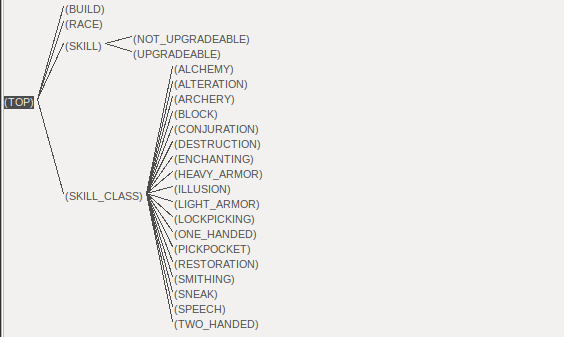
\includegraphics[scale=0.5]{taxonomy}
\end{figure}

\end{frame}

%------------------------------------------------

\begin{frame}
\frametitle{Tbox}

The Skill\_class is split into the existing 12 disjoint classes: \textit{Archery, Block, Heavy Armor, One-handed, Smithing, Two-handed, Alteration, Conjuration, Destruction, Enchanting, Illusion, Restoration, Alchemy, Light Armor, Lockpicking, Pickpocket, Sneak} and \textit{Speech}. These skill classes contain skills. Builds are paired with skill classes to tell what skill class is suitable for what build.
\newline
\newline
Skills can be either \textit{Upgradeable} or \textit{Not\_upgradeable}, these two traits are obviously disjoint between eachother. Above this, we need to model the pre-required skill, for which we use a role called \textit{hasSkillRequirement}. For the level requirement and perk description we use attributes.

\end{frame}

%------------------------------------------------

\begin{frame}
\frametitle{Abox}

Our Abox is mainly composed of instances of skills, then some races and some builds.
Instances of races and builds are simple, since they are then used to determine which skill class to invest in.

This can be seen in the tree structure in the images below. The skill is only the root, but since the skill requirement takes another skill as parameter, it extends until it reaches a "leaf skill".

\begin{figure}[h]
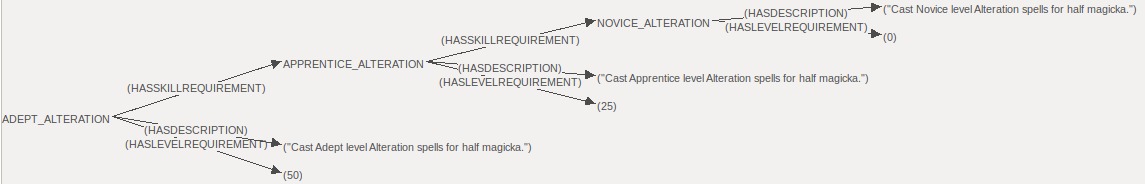
\includegraphics[scale=0.5]{abox_adept_alteration.png}
\end{figure}

\end{frame}

%------------------------------------------------

\begin{frame}
\frametitle{Queries}

The last thing we do as part of loading the ontology and before we run our queries is running all the rules with the \textit{run-all-rules} command. After this step, we can run our evaluation queries.
We check the consistency, the size, the expressivity of our ontology, and finally, we answer the competency question with some custom queries.

For more details and for the full code, please check the full documentation document.

\end{frame}

%------------------------------------------------

\begin{frame}
\Huge{\centerline{The End}}
\end{frame}

%----------------------------------------------------------------------------------------

\end{document} 